\documentclass[10pt,twocolumn]{article}

% ─── Packages ────────────────────────────────────────────────────────────────
\usepackage[T1]{fontenc}
\usepackage[utf8]{inputenc}
\usepackage{lmodern}
\usepackage{microtype}
\usepackage[top=1in,bottom=1in,left=0.85in,right=0.85in,columnsep=0.3in]{geometry}
\usepackage{amsmath,amssymb}
\usepackage{booktabs}
\usepackage{tabularx}
\usepackage{longtable}
\usepackage{array}
\usepackage{multirow}
\usepackage{graphicx}
\usepackage{xcolor}
\usepackage{tikz}
\usetikzlibrary{arrows.meta,positioning,shapes.geometric,fit,backgrounds,calc,decorations.pathreplacing}
\usepackage{pgfplots}
\pgfplotsset{compat=1.18}
\usepackage{listings}
\usepackage{caption}
\usepackage{subcaption}
\usepackage{enumitem}
\usepackage{fancyhdr}
\usepackage{titlesec}
\usepackage{hyperref}
\usepackage{cleveref}
\usepackage{cite}
\usepackage{url}
\usepackage{parskip}
\usepackage{setspace}
\usepackage{float}
\usepackage{flushend}
\usepackage{changepage}

% ─── Colors ──────────────────────────────────────────────────────────────────
\definecolor{agorblue}{RGB}{0,74,173}
\definecolor{agordark}{RGB}{15,23,42}
\definecolor{agorgray}{RGB}{100,116,139}
\definecolor{codebg}{RGB}{248,250,252}
\definecolor{codeframe}{RGB}{203,213,225}
\definecolor{rulecol}{RGB}{20,20,20}

% ─── Hyperref ────────────────────────────────────────────────────────────────
\hypersetup{
  colorlinks=true,
  linkcolor=agorblue,
  citecolor=agorblue,
  urlcolor=agorblue,
  pdftitle={Fusio: A Decentralized Protocol for Autonomous Agent Compute},
  pdfauthor={Ahmed Ali (Lord Amdal)}
}

% ─── Section formatting ───────────────────────────────────────────────────────
\titleformat{\section}{\large\bfseries\color{agordark}}{\thesection.}{0.5em}{}[\vspace{-2pt}\textcolor{rulecol}{\rule{\linewidth}{0.6pt}}]
\titleformat{\subsection}{\normalsize\bfseries\color{agordark}}{\thesubsection}{0.5em}{}
\titleformat{\subsubsection}{\small\bfseries\itshape\color{agorgray}}{\thesubsubsection}{0.5em}{}

\titlespacing{\section}{0pt}{8pt}{4pt}
\titlespacing{\subsection}{0pt}{6pt}{2pt}

% ─── Listings (code blocks) ───────────────────────────────────────────────────
\lstdefinestyle{protocolcode}{
  backgroundcolor=\color{codebg},
  frame=single,
  framerule=0.5pt,
  rulecolor=\color{codeframe},
  basicstyle=\ttfamily\scriptsize,
  keywordstyle=\bfseries\color{agorblue},
  commentstyle=\itshape\color{agorgray},
  stringstyle=\color{agorblue!70!black},
  breaklines=true,
  breakatwhitespace=false,
  tabsize=2,
  showstringspaces=false,
  captionpos=b,
  numbers=left,
  numberstyle=\tiny\color{agorgray},
  numbersep=4pt,
  xleftmargin=12pt,
  xrightmargin=4pt,
}
\lstset{style=protocolcode}

% ─── Caption style ────────────────────────────────────────────────────────────
\captionsetup{font=small,labelfont={bf,color=agordark},textfont=it,skip=4pt}

% ─── Header / Footer ─────────────────────────────────────────────────────────
\pagestyle{fancy}
\fancyhf{}
\fancyhead[L]{\small\textit{Fusio Protocol Whitepaper v0.9}}
\fancyhead[R]{\small\textit{Ali, A. (2026)}}
\fancyfoot[C]{\thepage}
\renewcommand{\headrulewidth}{0.4pt}
\renewcommand{\footrulewidth}{0pt}

% ─── Paragraph spacing ────────────────────────────────────────────────────────
\setlength{\parskip}{3pt}
\setlength{\parindent}{10pt}

% ─── Custom commands ──────────────────────────────────────────────────────────
\newcommand{\keyword}[1]{\textbf{#1}}
\newcommand{\proto}[1]{\texttt{\small #1}}
\newcommand{\fso}{\textsc{fso}}

% ─── Column balance helper ────────────────────────────────────────────────────
\newlength{\mycolwidth}
\setlength{\mycolwidth}{\columnwidth}

% ─── Suppress default \maketitle (we build title manually) ───────────────────
\renewcommand{\maketitle}{}

% ═════════════════════════════════════════════════════════════════════════════
\begin{document}
% ═════════════════════════════════════════════════════════════════════════════

\twocolumn[{%
  %% ── TITLE ──────────────────────────────────────────────────────────────
  \begin{center}
    \vspace*{4pt}
    {\fontsize{22}{26}\selectfont\bfseries Fusio}\\[8pt]
    {\large A Decentralized Protocol for Autonomous Agent Compute}\\[10pt]
    {\normalsize Ahmed Ali \quad (\textit{Lord Amdal})}\\[3pt]
    {\small \texttt{amdal.ali@oit.edu}}\\[3pt]
    {\small\color{agorgray} March 2026}
  \end{center}

  \vspace{10pt}
  \noindent\rule{\linewidth}{0.8pt}
  \vspace{6pt}

  %% ── ABSTRACT ────────────────────────────────────────────────────────────
  \begin{center}
    {\normalsize\bfseries Abstract}
  \end{center}
  \begin{adjustwidth}{0.5cm}{0.5cm}
  \normalsize
  The agora was the central public space of ancient Greek cities, a marketplace and meeting
  place governed by shared rules, open participation, visible transactions, and accountable
  actors with no single point of control. We are building its equivalent for the AI economy.
  \textbf{Fusio} is an open protocol that connects a \emph{requester} (a person with an AI model and a task) with a \emph{worker} (a person who contributes their computer to run that task). The exchange is governed by four non-overridable primitives: verified identity,
  matched routing, settled payment, and permanent receipt. The protocol is open source and
  owned by no entity. Any AI agent operating on Fusio can act, pay, and be held accountable
  without a human in the loop.

  \medskip\noindent
  \textbf{Keywords:}\enspace autonomous agents, decentralized compute, agentic infrastructure,
  browser automation, cryptographic accountability, token economics, AI protocols.
  \end{adjustwidth}

  \vspace{10pt}

  %% ── DISCLAIMER (framed, pale gray) ──────────────────────────────────────
  \noindent\colorbox{gray!12}{%
    \begin{minipage}{\dimexpr\linewidth-2\fboxsep\relax}
      \vspace{4pt}
      \small\itshape This document is published for review and comment by the technical
      community. It does not constitute an offer to sell securities. The \fso{} token
      described herein is a utility token. Readers should seek independent legal and
      financial advice before acting on any information contained herein.
      \vspace{4pt}
    \end{minipage}%
  }

  \vspace{12pt}
}]

% ─────────────────────────────────────────────────────────────────────────────
\section{Introduction}
\label{sec:intro}
% ─────────────────────────────────────────────────────────────────────────────

\subsection{The Original Agora}

The Greeks understood something most infrastructure builders forget: a marketplace is not
merely an economic mechanism; it is a public institution. It functions because everyone
can see what is happening, everyone knows the rules, and everyone is accountable to
everyone else. The agora was governed by shared rules, not controlled by any merchant or
guild. That model scaled across centuries and cultures because it was built on open
participation, visible transactions, accountable actors, and no single point of control. The
AI economy needs the same foundation.

\subsection{The Problem}

The history of computing is a history of collapsing asymmetries. The personal computer gave
individuals the power of institutions. The internet gave individuals the reach of publishers.
Cloud computing gave individuals the infrastructure of enterprises. We are at the beginning
of another such shift: AI models are becoming capable enough to perform knowledge work
that previously required teams of people.

However, there is a ceiling. AI models can think but they cannot act autonomously in the
world. They cannot open a browser and run a job for hours while the user is asleep, pay for
compute on behalf of their user, prove what they did, or maintain persistent identity. Every
agentic system built today requires a human to stay in the loop: to hold the credentials,
manage the infrastructure, and babysit execution. This is not a limitation of the models; it
is a limitation of the infrastructure underneath them.

\subsection{The Concrete Case}

Consider someone building a personal brand who wants an AI agent to: monitor social media
daily, identify trending topics, write articles in response, publish them to their blog, and
engage with comments. AI models available today are capable of each of these subtasks. Yet
to run this autonomously, the person must leave their own computer on, expose credentials
to whatever process is running, pay for compute from personal infrastructure, and operate
with no verifiable record of agent actions. The friction is prohibitive and the trust model is
unclear.

This pattern repeats across any autonomous task: managing business calendars, monitoring
competitors, processing incoming requests, executing research pipelines. Every one hits the
same ceiling. Fusio collapses this asymmetry.

\subsection{What Fusio Provides}

Fusio is not an AI model. It is not an application. It is a protocol: a set of rules allowing
different participants to interact predictably and trustworthily. The protocol defines four
things precisely (see \cref{tab:primitives}):
\begin{enumerate}[noitemsep,leftmargin=*,topsep=2pt]
  \item How an AI agent establishes a verified identity on the network;
  \item How a job is routed from a requester's AI model to a worker's computer;
  \item How the worker is paid in \fso{} when the job completes;
  \item How a signed receipt is written to an immutable on-chain log.
\end{enumerate}

\subsection{Why Now}

Three conditions align today that did not exist two years ago:
\begin{itemize}[noitemsep,leftmargin=*,topsep=2pt]
  \item \textbf{Model capability:} The reasoning required to plan and execute multi-step browser tasks exists in commercially available models. Model capability is no longer the binding constraint; infrastructure is.
  \item \textbf{Idle compute:} Hundreds of millions of personal computers sit idle for large portions of the day, aggregating compute that dwarfs any data center. A protocol enabling this compute to be safely contributed to a network is the missing layer.
  \item \textbf{Behavioral readiness:} People already rent their homes (Airbnb), cars (Turo), and time. Contributing idle compute to a network in exchange for tokens is a natural extension, provided the trust and safety model is credible.
\end{itemize}

% ─────────────────────────────────────────────────────────────────────────────
\section{Protocol Design}
\label{sec:design}
% ─────────────────────────────────────────────────────────────────────────────

Fusio is designed around a single core insight: \emph{identity and compute are not separable
in a trustworthy agentic system.} You cannot have verifiable compute without knowing who
authorized it; you cannot have accountable identity without knowing what actions it took.
The protocol treats these as a unified primitive.

\subsection{Participants}

Three participant classes interact in the protocol, as illustrated in \cref{fig:participants}.

\begin{figure}[H]
\centering
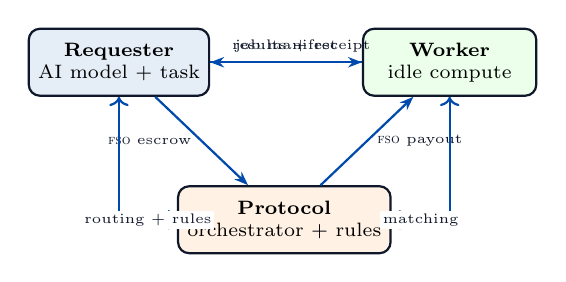
\begin{tikzpicture}[
  every node/.style={font=\scriptsize},
  box/.style={draw=agordark, rounded corners=4pt, fill=codebg, minimum width=2.2cm, minimum height=0.85cm, align=center, thick},
  arrow/.style={-{Stealth[length=5pt]}, thick, color=agorblue},
  doublearrow/.style={<->, thick, color=agorblue}
]
  \node[box, fill=agorblue!10] (req) at (0,0) {\textbf{Requester}\\AI model + task};
  \node[box, fill=green!8] (work) at (4.2,0) {\textbf{Worker}\\idle compute};
  \node[box, fill=orange!10] (proto) at (2.1,-2) {\textbf{Protocol}\\orchestrator + rules};

  \draw[arrow] (req) -- node[above,font=\tiny,color=agordark]{job manifest} (work);
  \draw[arrow] (work) -- node[above,font=\tiny,color=agordark,pos=0.4]{results + receipt} (req);
  \draw[arrow] (req) -- node[left,font=\tiny,color=agordark]{\fso{} escrow} (proto);
  \draw[arrow] (proto) -- node[right,font=\tiny,color=agordark]{\fso{} payout} (work);
  \draw[doublearrow] (proto) -- node[font=\tiny,color=agordark,fill=white,inner sep=1pt]{routing + rules} (req|-proto) -- (req);
  \draw[doublearrow] (proto) -- node[font=\tiny,color=agordark,fill=white,inner sep=1pt]{matching} (work|-proto) -- (work);
\end{tikzpicture}
\caption{Three participant classes and their interactions within the Fusio protocol.}
\label{fig:participants}
\end{figure}

\begin{itemize}[noitemsep,leftmargin=*,topsep=2pt]
  \item \textbf{Requester:} Connects an AI model to the Fusio network, submits jobs, pays in \fso{}, and receives results with signed receipts. The protocol does not touch the model, conversation, or user data.
  \item \textbf{Worker:} Runs the Fusio node software, contributes isolated compute and a residential IP address, earns \fso{}. Cannot observe job execution.
  \item \textbf{Protocol / Foundation:} Sets rules, runs the orchestrator, validates completions, issues receipts, manages token economics. Does not control individual jobs or user data.
\end{itemize}

\subsection{The Four Protocol Primitives}

Every network interaction flows through the four primitives in \cref{tab:primitives}. These are the \emph{only} things the protocol standardizes; everything else is implementation.

\begin{table}[H]
\centering
\caption{The Four Protocol Primitives}
\label{tab:primitives}
\renewcommand{\arraystretch}{1.35}
\begin{tabularx}{\columnwidth}{>{\bfseries\small}p{1.7cm} X}
\toprule
Primitive & Standardization Scope \\
\midrule
Agent Identity &
  Cryptographic keypair at registration. Public key is the on-chain address. Every job is signed by the requester's agent key; every worker receipt by the worker's key. Neither party can repudiate participation. \\[3pt]
Job Routing &
  Structured job manifest declaring required capability, budget, duration estimate, and stealth requirement. Orchestrator matches manifest to available workers and confirms before any job starts. \\[3pt]
Settlement &
  EVM smart contract holds requester's \fso{} in escrow at job start. Signed completion receipt triggers release. On failure, escrow is returned per fault classification. \\[3pt]
Accountability &
  Signed receipt containing: agent ID, worker ID (hashed), job hash, timestamps, action count, outcome, and cost. Written to an append-only on-chain log; cannot be altered or deleted. \\
\bottomrule
\end{tabularx}
\end{table}

\subsection{What the Protocol Does Not Standardize}

Fusio deliberately leaves the AI model, worker operating system, and application layer to implementers. A protocol that standardizes everything becomes a product. Fusio is a foundation upon which many products can be built, not a product itself.

% ─────────────────────────────────────────────────────────────────────────────
\section{How a Job Works}
\label{sec:job}
% ─────────────────────────────────────────────────────────────────────────────

\cref{fig:joblifecycle} provides the complete job lifecycle. The following subsections detail each phase using a running example: an AI agent that researches trending topics, writes a blog article, and publishes it.

\begin{figure}[H]
\centering
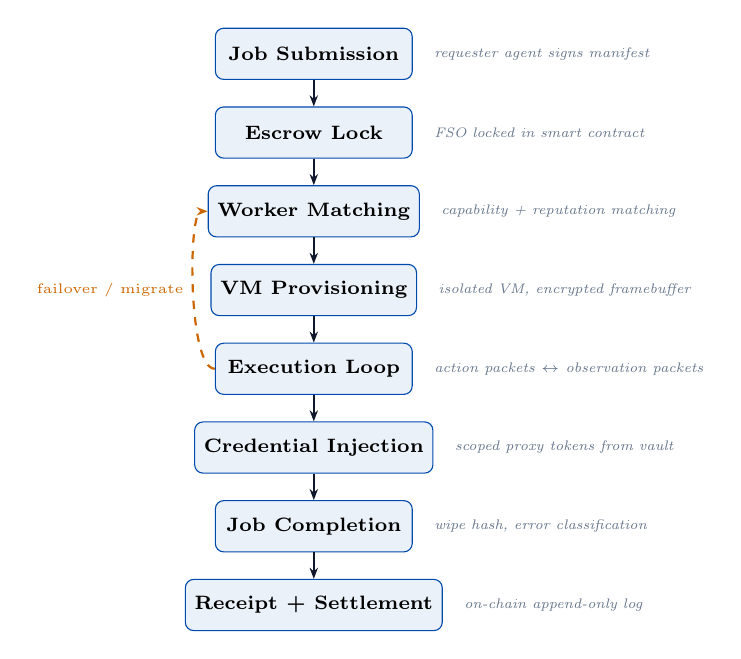
\begin{tikzpicture}[
  every node/.style={font=\scriptsize},
  step/.style={draw=agordark, rounded corners=3pt, fill=codebg, minimum width=2.5cm, minimum height=0.65cm, align=center},
  phase/.style={draw=agorblue, rounded corners=3pt, fill=agorblue!8, minimum width=2.5cm, minimum height=0.65cm, align=center, font=\scriptsize\bfseries},
  arr/.style={-{Stealth[length=4pt]}, thick, color=agordark},
  note/.style={font=\tiny\itshape, color=agorgray}
]
  \node[phase] (submit)  at (0,0)     {Job Submission};
  \node[phase] (escrow)  at (0,-1.0)  {Escrow Lock};
  \node[phase] (match)   at (0,-2.0)  {Worker Matching};
  \node[phase] (vm)      at (0,-3.0)  {VM Provisioning};
  \node[phase] (exec)    at (0,-4.0)  {Execution Loop};
  \node[phase] (cred)    at (0,-5.0)  {Credential Injection};
  \node[phase] (complete)at (0,-6.0)  {Job Completion};
  \node[phase] (receipt) at (0,-7.0)  {Receipt + Settlement};

  \foreach \a/\b in {submit/escrow, escrow/match, match/vm, vm/exec, exec/cred, cred/complete, complete/receipt}
    \draw[arr] (\a) -- (\b);

  % Side annotations
  \node[note, right=0.15cm of submit]   {requester agent signs manifest};
  \node[note, right=0.15cm of escrow]   {FSO locked in smart contract};
  \node[note, right=0.15cm of match]    {capability + reputation matching};
  \node[note, right=0.15cm of vm]       {isolated VM, encrypted framebuffer};
  \node[note, right=0.15cm of exec]     {action packets $\leftrightarrow$ observation packets};
  \node[note, right=0.15cm of cred]     {scoped proxy tokens from vault};
  \node[note, right=0.15cm of complete] {wipe hash, error classification};
  \node[note, right=0.15cm of receipt]  {on-chain append-only log};

  % Failover arrow
  \draw[-{Stealth[length=4pt]}, thick, color=orange!80!black, dashed]
    (exec.west) .. controls (-1.6,-4) and (-1.6,-2) .. node[left,font=\tiny,color=orange!80!black]{failover / migrate} (match.west);
\end{tikzpicture}
\caption{Complete job lifecycle in the Fusio protocol. Orange dashed arrow indicates the migration path on worker node failure.}
\label{fig:joblifecycle}
\end{figure}

\subsection{Job Submission}

The requester's AI model signs a structured job manifest with the requester's agent private key. The orchestrator validates the manifest (identity record, category prohibition list, balance sufficiency) and locks the declared amount in escrow.

\begin{lstlisting}[language={},caption={Job Manifest Structure},label={lst:manifest}]
job_manifest {
  job_id:           uuid,
  agent_id:         requester_public_key,
  agent_signature:  signs_entire_manifest,
  capability:       'browser.full',
  stealth_required: 'vm_stealth',
  estimated_minutes: 45,
  max_price_fso:    2.00,
  browser:          'chromium',
  declared_purpose: 'content research and publishing',
  category:         'content.creation',
  memory_policy:    'persistent',
  failover_policy:  'migrate'
}
\end{lstlisting}

\subsection{Worker Matching}

Workers continuously broadcast capability profiles to the orchestrator. The orchestrator matches job manifests against available profiles on three axes: (1) declared capability, (2) reputation score, and (3) price. On confirmation, the worker's node software spins up an isolated VM. The worker receives no information beyond what is needed to provision the VM: not the declared purpose, requester identity, or job instructions.

\subsection{The Execution Loop}

Execution proceeds as a request/observation loop (\cref{fig:execloop}) until job completion, budget exhaustion, or a failure condition.

\begin{figure}[H]
\centering
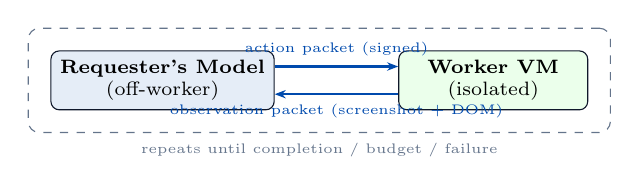
\begin{tikzpicture}[
  every node/.style={font=\scriptsize},
  box/.style={draw=agordark, rounded corners=3pt, fill=codebg, minimum width=2.4cm, minimum height=0.7cm, align=center},
  arr/.style={-{Stealth[length=4pt]}, thick, color=agorblue}
]
  \node[box, fill=agorblue!10] (model) at (0,0)    {\textbf{Requester's Model}\\(off-worker)};
  \node[box, fill=green!8]     (vm)    at (4.2,0)  {\textbf{Worker VM}\\(isolated)};

  \draw[arr, transform canvas={yshift=5pt}]
    (model) -- node[above,font=\tiny]{action packet (signed)} (vm);
  \draw[arr, transform canvas={yshift=-5pt}]
    (vm) -- node[below,font=\tiny]{observation packet (screenshot + DOM)} (model);

  \node[draw=agorgray, dashed, rounded corners, fit=(model)(vm),
        inner sep=8pt, font=\tiny\itshape, label={[font=\tiny,color=agorgray]below:repeats until completion / budget / failure}] {};
\end{tikzpicture}
\caption{The execution loop. The requester's model never runs on the worker's machine; only action instructions and screen observations cross the boundary.}
\label{fig:execloop}
\end{figure}

The protocol packet formats are defined as follows:

\begin{lstlisting}[language={},caption={Action and Observation Packet Formats},label={lst:packets}]
action_packet {
  job_id:   uuid,
  step:     integer,
  action:   'click' | 'type' | 'navigate'
          | 'scroll' | 'screenshot' | 'wait',
  target:   {x: number, y: number} | url,
  value:    string | null,
  signed_by: requester_agent_key
}

observation_packet {
  job_id:    uuid,
  step:      integer,
  screenshot: base64_image,
  dom_state:  compressed_semantic_description,
  signed_by:  worker_key
}
\end{lstlisting}

\subsection{VM Isolation}

The VM enforces isolation at four independent layers, summarized in \cref{tab:isolation}. Isolation is enforced by architecture, not policy.

\begin{table}[H]
\centering
\caption{VM Isolation Layers}
\label{tab:isolation}
\renewcommand{\arraystretch}{1.3}
\begin{tabularx}{\columnwidth}{>{\bfseries\small}p{1.8cm} X}
\toprule
Layer & Mechanism \\
\midrule
Screen output & Encrypted framebuffer; worker host OS cannot read screen content \\
Network & All traffic exits through encrypted tunnel to Fusio relay before the open internet; worker cannot observe visited sites \\
Credentials & Injected into a hardware enclave; never appear in readable memory outside the enclave \\
Disk & Ephemeral; cryptographically wiped on job completion; wipe hash included in completion receipt \\
\bottomrule
\end{tabularx}
\end{table}

\noindent Workers observe only: CPU usage, RAM usage, job duration, and \fso{} earnings.

\subsection{The Browser Identity Stack}

Jobs interacting with automation-detection sites require a browser environment that appears as a real user session. The protocol's browser identity stack applies the following to every VM session:

\begin{itemize}[noitemsep,leftmargin=*,topsep=2pt]
  \item User-agent string reflects a current real browser release
  \item Platform string, screen resolution, timezone, language, and hardware concurrency drawn from the worker's \emph{actual} host machine (real values, not fabricated)
  \item WebDriver flag explicitly disabled
  \item Canvas fingerprint entropy randomized per session but stable within a session
  \item Destination sites see a real residential IP via the worker's connection through the encrypted tunnel
\end{itemize}

This approach is more resilient than fabricated fingerprints because the underlying hardware signals are genuine.

\subsection{Job Memory and State}

Long-running jobs persist state across steps through three memory tiers:

\begin{table}[H]
\centering
\caption{Job Memory Tiers}
\label{tab:memory}
\renewcommand{\arraystretch}{1.3}
\begin{tabularx}{\columnwidth}{>{\bfseries\small}p{1.6cm} X}
\toprule
Tier & Description \\
\midrule
Working memory & Agent context within a single execution session; held in encrypted VM memory \\
Step memory & Structured snapshot of job progress written to the Fusio relay at configurable intervals; enables migration without restart \\
Agent memory & Persistent storage owned by the requester's agent identity; maintained across jobs; accumulates knowledge about requester preferences and history \\
\bottomrule
\end{tabularx}
\end{table}

\subsection{Failover and Migration}

The orchestrator monitors a heartbeat signal from every active job. Absence for 30 seconds triggers migration: the orchestrator loads the most recent step snapshot, finds a new eligible worker, and resumes from the last confirmed step. \emph{Credentials are never included in the step snapshot.} The new worker receives a fresh credential token issued by the vault; the original token is revoked.

% ─────────────────────────────────────────────────────────────────────────────
\section{Credentials and the Front Desk Agent}
\label{sec:credentials}
% ─────────────────────────────────────────────────────────────────────────────

Handling credentials in a decentralized system where workers are unknown and untrusted is the hardest security problem the protocol faces. Passing credentials in the job manifest is unacceptable: workers would see plaintext secrets.

\subsection{The Vault Model}

The vault is controlled by the requester's principal identity. It never releases raw credentials to workers. Instead, it issues \emph{short-lived scoped proxy tokens} at job start; each token grants access to a specific service, for a specific scope, for the duration of a specific job. The token lifecycle is illustrated in \cref{fig:vault}.

\begin{figure}[H]
\centering
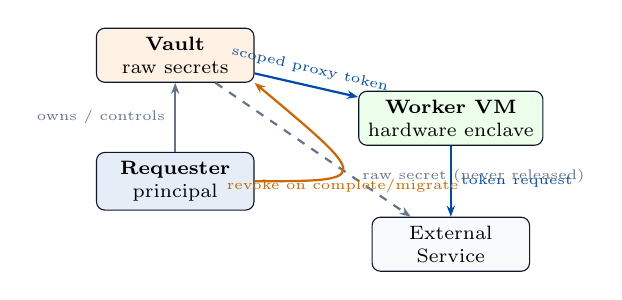
\begin{tikzpicture}[
  every node/.style={font=\scriptsize},
  box/.style={draw=agordark, rounded corners=3pt, fill=codebg, minimum width=2cm, minimum height=0.65cm, align=center},
  arr/.style={-{Stealth[length=4pt]}, thick}
]
  \node[box, fill=orange!10] (vault)  at (0,0)   {\textbf{Vault}\\raw secrets};
  \node[box, fill=agorblue!10] (req)  at (0,-1.6) {\textbf{Requester}\\principal};
  \node[box, fill=green!8]  (vm)     at (3.5,-0.8) {\textbf{Worker VM}\\hardware enclave};
  \node[box, fill=codebg]   (svc)    at (3.5,-2.4) {External\\Service};

  \draw[arr, color=agorgray] (req) -- node[left,font=\tiny]{owns / controls} (vault);
  \draw[arr, color=agorblue] (vault) -- node[above,font=\tiny,sloped]{scoped proxy token} (vm);
  \draw[arr, color=agorblue] (vm) -- node[right,font=\tiny]{token request} (svc);
  \draw[arr, color=agorgray, dashed] (vault) -- node[right,font=\tiny,pos=0.7]{raw secret (never released)} (svc);
  \draw[arr, color=orange!80!black] (req.east) .. controls (2.5,-1.6) .. node[below,font=\tiny,color=orange!80!black]{revoke on complete/migrate} (vault.south east);
\end{tikzpicture}
\caption{Vault model: raw credentials are never released to workers. Scoped proxy tokens expire with the job; on migration, the old token is revoked before the new one is issued.}
\label{fig:vault}
\end{figure}

If a worker's machine is compromised, the attacker obtains only an expired scoped token tied to a job that no longer exists.

\subsection{The Front Desk Agent}

The front desk agent is a lightweight onboarding flow built into the Fusio client. Before a credentialed job starts, it checks the vault. If credentials are missing, it presents a guided setup flow:

\begin{itemize}[noitemsep,leftmargin=*,topsep=2pt]
  \item \textbf{OAuth services:} Opens the provider's consent screen in the requester's browser. The access token goes directly to the vault without passing through intermediate application state.
  \item \textbf{API key services:} The requester pastes the key into an encrypted input field. It is encrypted on entry and stored in the vault. The raw key never appears in readable application memory.
\end{itemize}

The front desk agent validates each credential with a test call before job start. This prevents spending \fso{} on jobs that would fail immediately due to credential problems.

% ─────────────────────────────────────────────────────────────────────────────
\section{Error Handling and Worker Protection}
\label{sec:errors}
% ─────────────────────────────────────────────────────────────────────────────

\subsection{Error Classification}

Every job failure is classified by fault before any penalty or refund is applied. \cref{tab:errors} specifies the five fault classes and their consequences.

\begin{table}[H]
\centering
\caption{Error Classification and Consequences}
\label{tab:errors}
\renewcommand{\arraystretch}{1.35}
\begin{tabularx}{\columnwidth}{>{\bfseries\small}p{1.5cm} p{1.7cm} X}
\toprule
Class & Example & Consequence \\
\midrule
Worker fault & Node crashes mid-job & Worker reputation penalty. Job migrates. Partial \fso{} returned. \\
Requester fault & Bad instructions cause infinite loop & No worker penalty. \fso{} spent for time used. \\
External & Site blocks browser session & No penalty to either party. Job requeued. Requester refunded. \\
Environmental & Site UI changed mid-job & No penalty. Logged as environmental failure. Requester refunded. \\
Credential & OAuth token expired during job & No worker penalty. Job paused. Requester notified to refresh. \\
\bottomrule
\end{tabularx}
\end{table}

Classification is determined by the error packet submitted at termination, containing: failure class, step at failure, screenshot of screen state, and recovery recommendation.

\subsection{Worker Legal Protection}

A worker contributing compute to the network is a passive infrastructure provider. They do not author job instructions, cannot see job purpose, and cannot observe execution, enforced by protocol architecture, not policy.

Every job is cryptographically signed by the requester's agent identity. The signature appears in the job manifest, in every action packet, and in the completion receipt. The evidence chain in the protocol audit log leads to the requester. The worker's contribution to that job is documented solely as compute provision. Workers agree to participation terms that establish their role as compute providers and commit them to cooperating with valid legal process; in return, the protocol commits to producing requester identity evidence should a worker's compute be implicated in a harmful job.

\noindent\textit{Note: This framework is designed to mirror the legal protections cloud compute providers enjoy in most jurisdictions. Workers should review participation terms for their specific legal jurisdiction.}

\subsection{Prohibited Job Categories}

The orchestrator enforces a pre-execution prohibition list:
\begin{itemize}[noitemsep,leftmargin=*,topsep=2pt]
  \item Jobs targeting financial institution login flows
  \item Jobs submitting PII belonging to third parties
  \item Jobs interacting with domains associated with known fraud patterns
  \item Jobs executing high-value purchase flows without explicit requester authorization
\end{itemize}
This screening is logged and cryptographically provable; workers are protected before execution begins.

% ─────────────────────────────────────────────────────────────────────────────
\section{Token Economics}
\label{sec:token}
% ─────────────────────────────────────────────────────────────────────────────

The \fso{} token is the native utility token of the Fusio protocol. Its primary purpose is settling economic transactions between requesters and workers globally, instantly, and without a common financial intermediary. The name ``Fusio'' derives from the Latin 	extit{fusio} (fusion, convergence, a merging of flows) and is the common medium that allows strangers to transact without a bank, platform, or middleman.

\subsection{Why a Native Token}

Job sizes on the Fusio network are small: a 15-minute browser session may cost fractions of a cent in compute terms; a long-running research job a few dollars. These transaction sizes are impractical in fiat currency: payment processing fees would exceed job costs for small jobs, and international wire transfers are too slow and expensive for micropayments to workers in other countries. A native token settles instantly, globally, and at negligible per-transaction cost.

\subsection{Token Utility}

\fso{} utility flows through four channels:
\begin{itemize}[noitemsep,leftmargin=*,topsep=2pt]
  \item \textbf{Requesters} acquire \fso{} to pay for jobs
  \item \textbf{Workers} earn \fso{} by completing jobs
  \item \textbf{Service providers} stake \fso{} to list capabilities (stake slashed on consistent unavailability)
  \item \textbf{Foundation} earns \fso{} through network fees on settled transactions
\end{itemize}

\fso{} is not a speculative instrument. Its value is grounded in network utility: as more jobs run, more \fso{} is required. Token value tracks genuine network activity rather than speculation about future activity.

\subsection{Minting and Supply}

The minting schedule is defined in the protocol specification and controlled by the foundation within hardcoded limits. Changes to the minting schedule require a protocol upgrade following the governance process (\cref{sec:governance}). Network fees split between the foundation treasury and a protocol reserve, which funds node operator incentives during early growth when organic job volume is insufficient to attract workers without supplemental rewards.

\subsection{Worker Reward Formula}

Worker earnings are calculated from three factors:

\begin{equation}
  \text{FSO}_{\text{earned}} = R_{\text{base}} \times M_{\text{rep}} \times F_{\text{complexity}}
  \label{eq:reward}
\end{equation}

\noindent where:
\begin{itemize}[noitemsep,leftmargin=*,topsep=2pt]
  \item $R_{\text{base}}$ is the base job rate agreed in the manifest at match time
  \item $M_{\text{rep}} \in [0.8,\ 1.2]$ is the reputation multiplier (0.8 for new workers; 1.2 for established workers with strong completion records)
  \item $F_{\text{complexity}}$ accounts for job duration and total action count
\end{itemize}

New workers start at $M_{\text{rep}} = 0.8$ and earn upward through successful completions, creating a natural quality gradient in the worker pool without manual review.

% ─────────────────────────────────────────────────────────────────────────────
\section{The Application Layer}
\label{sec:app}
% ─────────────────────────────────────────────────────────────────────────────

The protocol defines the rules. The application is what people actually use. The first application built on the Fusio protocol is the Fusio Client, operated by the founding organization. The protocol is designed so that any party can build additional applications on it.

\subsection{The Fusio Client}

The Fusio client is a chat application. The requester connects it to any AI model (Claude, ChatGPT, Gemini, a locally running model, or any model exposing a compatible API). They describe their goal in natural language. When the model determines that the task requires browser automation or off-device compute, it submits a job to the Fusio network. The requester need not understand the protocol.

\subsection{Worker Mode}

The same client application runs in worker mode. The operator configures: how much compute to contribute, availability hours, and accepted job categories. The application runs the Fusio node software in the background. Jobs are matched and executed automatically. \fso{} earnings accumulate in the worker's wallet. A worker who leaves their machine available overnight earns meaningful \fso{} without active involvement beyond initial setup.

\subsection{Live Session Visibility}

Requesters can watch jobs in real time. The Fusio client provides a live session view streaming the job screen from the worker's VM over an authenticated WebRTC connection \cite{w3c_webrtc}. The stream is not recorded, not stored, and is available only to the authenticated requester for the duration of the job.

Requesters may request control of the session: the agent pauses, keyboard and mouse inputs are forwarded to the VM, and on handback the agent re-observes the current screen state and continues its plan from where it left off, incorporating the requester's changes.

% ─────────────────────────────────────────────────────────────────────────────
\section{Governance}
\label{sec:governance}
% ─────────────────────────────────────────────────────────────────────────────

The Fusio protocol is not owned by its founding organization. The founding organization is the initial maintainer and operator of the reference implementation and the first hosted network. The protocol itself belongs to no one, and the rules for changing it are defined in the protocol rather than controlled by any single party.

\subsection{The Foundation}

The Fusio Foundation is an independent nonprofit stewarding the open source protocol. Funded by network fees and the foundation's allocation of \fso{} from the token treasury. Its mandate: maintain the protocol specification, publish the reference implementation, fund core engineering, and coordinate the upgrade process. The foundation does not control individual jobs, user data, worker nodes, or the \fso{} token price.

\subsection{Protocol Upgrades}

Any participant may propose a protocol upgrade by submitting a Protocol Improvement Proposal (PIP) to the foundation's public repository. The process is:
\begin{enumerate}[noitemsep,leftmargin=*,topsep=2pt]
  \item Technical review by the core engineering team for soundness
  \item Minimum 30-day public comment period upon passing technical review
  \item Vote by the foundation's technical committee
  \item Approved proposals activated at a scheduled block height
\end{enumerate}

Changes to the token minting schedule, fee structure, or governance process itself require a supermajority of the technical committee and a 60-day comment period; these parameters are treated as constitutional.

\subsection{Transition to Community Governance}

The foundation model is appropriate for a new protocol requiring clear leadership and fast decision-making in response to real usage. The Fusio Foundation intends to transition toward token-holder governance as the protocol matures, driven by ecosystem readiness rather than an arbitrary schedule. The foundation will publish a governance maturity framework defining conditions for each stage of decentralization.

% ─────────────────────────────────────────────────────────────────────────────
\section{Competitive Context}
\label{sec:competitive}
% ─────────────────────────────────────────────────────────────────────────────

\cref{tab:competitive} positions Fusio relative to the most relevant existing systems. The combination Fusio offers (decentralized browser-based agent compute with identity, settlement, and accountability built into the protocol) has no direct equivalent today.

\begin{table}[H]
\centering
\caption{Competitive Landscape}
\label{tab:competitive}
\renewcommand{\arraystretch}{1.4}
\begin{tabularx}{\columnwidth}{>{\bfseries\small}p{1.7cm} X}
\toprule
System & Relationship to Fusio \\
\midrule
LangGraph CUA + Scrapybara &
  Closest existing pattern. LangGraph provides the agent loop; Scrapybara provides centralized cloud VMs. Fusio replaces Scrapybara with a decentralized worker network and adds identity, settlement, and accountability that this pattern lacks. \\[3pt]
Akash Network &
  Decentralized compute for containers and servers. No browser automation, no agent identity, no job-level accountability. Fusio is specifically designed for the browser-based agentic use case. \\[3pt]
AWS + browser automation &
  Centralized, expensive for small jobs, no worker economy, no token settlement, not accessible to the public as a compute contributor. \\[3pt]
Golem / iExec &
  Decentralized compute marketplaces for general computation. Not designed for browser-based agent tasks; no action packet protocol or browser identity stack equivalent. \\[3pt]
0G Labs &
  Decentralized AI infrastructure focused on inference, storage, and on-chain settlement. Fusio's specific contribution is the browser-based computer-use layer and the human worker economy that makes real residential IPs and real machine fingerprints available. \\
\bottomrule
\end{tabularx}
\end{table}

The closest alternatives are either centralized, not designed for agents, or missing the accountability layer that makes autonomous agent actions safe enough to trust at scale.

% ─────────────────────────────────────────────────────────────────────────────
\section{Roadmap}
\label{sec:roadmap}
% ─────────────────────────────────────────────────────────────────────────────

The roadmap is organized around questions each phase must answer, rather than feature lists. \cref{fig:roadmap} provides a visual overview.

\begin{figure}[H]
\centering
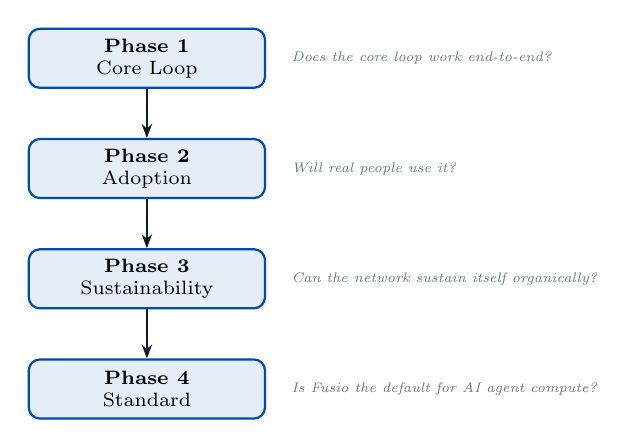
\begin{tikzpicture}[
  every node/.style={font=\scriptsize},
  phase/.style={draw=agorblue, fill=agorblue!10, rounded corners=4pt,
                minimum width=3.0cm, minimum height=0.75cm, align=center, thick},
  q/.style={font=\tiny\itshape, color=agorgray},
  arr/.style={-{Stealth[length=5pt]}, thick, color=agordark}
]
  \node[phase] (p1) at (0,0)    {\textbf{Phase 1}\\Core Loop};
  \node[phase] (p2) at (0,-1.4) {\textbf{Phase 2}\\Adoption};
  \node[phase] (p3) at (0,-2.8) {\textbf{Phase 3}\\Sustainability};
  \node[phase] (p4) at (0,-4.2) {\textbf{Phase 4}\\Standard};

  \draw[arr] (p1) -- (p2);
  \draw[arr] (p2) -- (p3);
  \draw[arr] (p3) -- (p4);

  \node[q, right=0.2cm of p1] {Does the core loop work end-to-end?};
  \node[q, right=0.2cm of p2] {Will real people use it?};
  \node[q, right=0.2cm of p3] {Can the network sustain itself organically?};
  \node[q, right=0.2cm of p4] {Is Fusio the default for AI agent compute?};
\end{tikzpicture}
\caption{Four-phase roadmap organized by the question each phase must answer.}
\label{fig:roadmap}
\end{figure}

\subsection{Phase 1: Does the Core Loop Work?}

Goal: a working end-to-end demonstration. One requester, one AI model, one job, one worker, one signed receipt. The target demo is blog research and publishing, complex enough to validate the protocol under real conditions. Deliverables: four protocol primitives in the reference implementation; Fusio orchestrator on founding-organization infrastructure; node software installable on Linux and macOS; action packet format finalized and published; \fso{} token on testnet; demo recorded and published.

\subsection{Phase 2: Will People Use It?}

Goal: real users running real jobs. Founding-organization worker nodes provide baseline availability while the organic worker community grows. The client application is polished for non-technical users; the front desk agent handles credential onboarding without requiring OAuth knowledge; worker onboarding completes in under five minutes. Deliverables: public beta client; worker onboarding flow; live session viewer; reputation system active; \fso{} on mainnet; first ten third-party jobs run by external parties.

\subsection{Phase 3: Can the Network Sustain Itself?}

Goal: organic worker participation exceeds founding-organization node capacity. Job categories expand beyond browser automation to other compute types built by the community. Deliverables: agent-to-agent job chaining; enterprise compliance tier with enhanced audit exports; open governance transition beginning; Protocol Improvement Proposal process active with meaningful community participation.

\subsection{Phase 4: Is Fusio the Standard?}

Goal: Fusio becomes the default method for AI agents to request and execute compute. This requires: integration into major AI frameworks enabling developers to reach the Fusio network without understanding the protocol directly; agent identity standard adopted beyond the Fusio network so identity and history are portable across systems; governance sufficiently decentralized that the protocol's future does not depend on any single organization.

% ─────────────────────────────────────────────────────────────────────────────
\section{Conclusion}
\label{sec:conclusion}
% ─────────────────────────────────────────────────────────────────────────────

The agora worked because it was designed around a simple truth: when people can transact in the open, under shared rules, with identities known and actions visible, trust scales, commerce grows, and the community becomes more than the sum of its members. The AI economy is at the beginning of the same kind of moment. The models exist. The compute exists. The demand is real and growing. What is missing is the open space where it can all come together safely, fairly, and at scale.

Fusio is that space: four primitives, open source, governed by a foundation that intends to decentralize as the ecosystem matures. The token economics are grounded in genuine utility. The worker protection model is as strong as the law allows. The privacy guarantees are enforced by architecture rather than policy. Real people getting paid for compute they already own. Real agents doing real work in the world.

\begin{center}
\textit{Any AI agent can act, pay, and be held accountable, without a human in the loop.}
\end{center}

% ─────────────────────────────────────────────────────────────────────────────
\section*{Acknowledgments}
\label{sec:ack}
% ─────────────────────────────────────────────────────────────────────────────

The author acknowledges the open-source communities behind the Ethereum protocol, LangChain/LangGraph, Playwright, and the broader decentralized compute research ecosystem, whose prior work provides the technical foundation upon which Fusio is built.

% ─────────────────────────────────────────────────────────────────────────────
\begin{thebibliography}{10}

\bibitem{nakamoto2008}
S.\ Nakamoto, ``Bitcoin: A Peer-to-Peer Electronic Cash System,'' 2008.
\url{https://bitcoin.org/bitcoin.pdf}

\bibitem{buterin2014}
V.\ Buterin, ``Ethereum: A Next-Generation Smart Contract and Decentralized Application Platform,'' 2014.
\url{https://ethereum.org/whitepaper/}

\bibitem{langchain2025}
LangChain AI, ``LangGraph Computer Use Agent,'' GitHub, 2025.
\url{https://github.com/langchainai/langgraph-cua-py}

\bibitem{cloudact2018}
U.S. Congress, ``Clarifying Lawful Overseas Use of Data (CLOUD) Act,'' Public Law 115-141, 2018.
\url{https://www.congress.gov/bill/115th-congress/house-bill/4943}

\bibitem{intel2023}
Intel Corporation, ``Software Guard Extensions Developer Guide,'' 2023.
\url{https://www.intel.com/sgx}

\bibitem{w3c_webrtc}
World Wide Web Consortium, ``WebRTC 1.0: Real-Time Communication Between Browsers,'' 2024.
\url{https://www.w3.org/TR/webrtc/}

\bibitem{playwright2025}
Playwright Project, ``Browser Automation Documentation,'' 2025.
\url{https://playwright.dev}

\bibitem{hansen2006}
M.H.\ Hansen, \textit{Polis: An Introduction to the Ancient Greek City-State}.
Oxford University Press, 2006.

\end{thebibliography}

% ─────────────────────────────────────────────────────────────────────────────
\onecolumn
\appendix
% ─────────────────────────────────────────────────────────────────────────────

\section{Glossary}
\label{app:glossary}

\begin{longtable}{>{\bfseries}p{3.2cm} p{10cm}}
\toprule
Term & Definition \\
\midrule
\endhead
Agent & An AI system operating on the Fusio network with a registered identity, a wallet, and the ability to submit and pay for jobs. \\[4pt]
Principal & The human or organization that owns an agent and is legally accountable for its actions. \\[4pt]
Requester & A principal who submits jobs to the Fusio network for execution on worker nodes. \\[4pt]
Worker & A person who runs the Fusio node software and contributes their computer's resources to the network in exchange for \fso{}. \\[4pt]
\fso{} & Fusio token. The native EVM-based utility token used for all economic transactions on the protocol: job payments, worker earnings, provider staking, and network fees. \\[4pt]
Job manifest & The signed document submitted by a requester that declares what a job needs and authorizes its execution. \\[4pt]
Action packet & The structured instruction format transmitted from the requester's AI model to the worker's VM defining a single browser or computer action. \\[4pt]
Observation packet & The structured response from the worker's VM containing a screenshot and semantic screen description. \\[4pt]
Front desk agent & The onboarding flow that collects and validates credentials before a job starts. \\[4pt]
Step snapshot & A serialized record of a job's progress written to the relay at regular intervals, enabling migration without restarting from the beginning. \\[4pt]
Vault & The encrypted credential store controlled by the requester's principal identity. Issues scoped proxy tokens to workers rather than raw credentials. \\[4pt]
Escrow & The smart contract that holds a requester's \fso{} during job execution and releases it to the worker on verified completion. \\[4pt]
Wipe hash & A cryptographic proof included in the worker's completion receipt confirming that the VM disk was securely destroyed after the job ended. \\[4pt]
Reputation score & A normalized score computed from a worker's history of successful job completions. Maps to an earnings multiplier $M_{\text{rep}} \in [0.8,\ 1.2]$: new workers start at 0.8 and earn upward through verified completions. \\[4pt]
Protocol Improvement Proposal (PIP) & A formal document proposing a change to the Fusio protocol specification, subject to the governance process in \cref{sec:governance}. \\
\bottomrule
\end{longtable}

\section{Action Packet Reference}
\label{app:actionpacket}

The following action types are defined in the initial protocol specification. Additional types may be added through the PIP process.

\begin{longtable}{>{\ttfamily\small}p{2.0cm} p{4.5cm} p{6.5cm}}
\toprule
Action & Parameters & Description \\
\midrule
\endhead
navigate & \texttt{url: string} & Navigate the browser to a URL. \\[3pt]
click & \texttt{x: number, y: number} & Click at the specified screen coordinates. \\[3pt]
type & \texttt{value: string} & Type text at the current cursor position. \\[3pt]
scroll & \texttt{direction: up|down|left|right,} \newline \texttt{amount: number} & Scroll the page in the specified direction by the specified amount. \\[3pt]
screenshot & \textit{(none)} & Capture the current screen state and return an observation packet. \\[3pt]
wait & \texttt{ms: number} & Wait for the specified number of milliseconds. \\[3pt]
key & \texttt{key: string} & Press a keyboard key or combination. \\[3pt]
select & \texttt{x: number, y: number,} \newline \texttt{value: string} & Select a dropdown option at the specified coordinates. \\[3pt]
hover & \texttt{x: number, y: number} & Move the mouse to coordinates without clicking. \\
\bottomrule
\end{longtable}

\end{document}
